\documentclass[10pt]{beamer}

\usepackage{graphicx}
%\usepackage{amsmath}
\graphicspath{ {images/} }

\usetheme[progressbar=frametitle]{metropolis}
\usepackage{appendixnumberbeamer}

\usepackage{booktabs}
\usepackage[scale=2]{ccicons}

\usepackage{pgfplots}
\usepgfplotslibrary{dateplot}

\usepackage{xspace}
\newcommand{\themename}{\textbf{\textsc{metropolis}}\xspace}

\pgfplotsset{soldot/.style={color=brown,only marks,mark=*}} \pgfplotsset{holdot/.style={color=brown,fill=white,only marks,mark=*}}

\usepackage{amssymb}
\usepackage{amsmath}
\usepackage{amsthm}
\usepackage{verbatim}
\usepackage{booktabs}
\usepackage{mathrsfs}
\usepackage{stmaryrd}


\title{R\'eseau de neurones artificiels}
\subtitle{Reconnaissance de caract\`eres}
% \date{\today}
\date{}
\author{\textsc{L\'opez Herranz Daniel}}

\institute{Lyc\'ee Saint-Louis}
%\titlegraphic{\hfill\includegraphics[height=1.5cm]{logo.pdf}}

\begin{document}

\maketitle

\begin{frame}{Sommaire}
  \setbeamertemplate{section in toc}[sections numbered]
  \tableofcontents[hideallsubsections]
\end{frame}

\section{Introduction}

%IA, présentation rapide => réseau de neurones
\begin{frame}[fragile]{Pourquoi un r\'eseau de neurones artificiels?}
	\begin{itemize}
		\item Algorithme puissant
		\item Vaste domaine d'appliquabilit\'e
	\end{itemize}
\end{frame}

\section{Cerveau biologique}

\begin{frame}{Neurone}
	$ $\\$ $
	\begin{figure}
  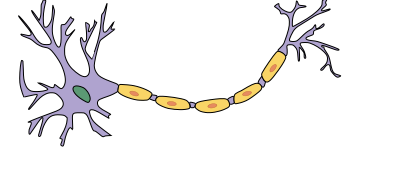
\includegraphics[scale=0.6]{neuron2}
	\centering
	\end{figure}
	Un \textbf{neurone} est constitu\'e:
	%\begin{itemize}
		%\item des dendrites
		%\item du noyau
		%\item de l'axone
		%\item des zones synaptiques
	%\end{itemize}

  \begin{columns}[T,onlytextwidth]
    \column{0.3\textwidth}
      \begin{itemize}
        \item des dendrites \item du noyau
      \end{itemize}

    \column{0.4\textwidth}
      \begin{itemize}
        \item de l'axone \item des zones synaptiques
      \end{itemize}
  \end{columns}
	$ $\\
	Il transmet un signal des dendrites aux zones synaptiques
\end{frame}

{
    \metroset{titleformat frame=smallcaps}
\begin{frame}{Fonctionnement}
	\begin{figure}
  \includegraphics[scale=0.3]{déclencher}
	\centering
	\end{figure}
	Le potentiel d'action suit la \textbf{loi du tout ou rien}
\end{frame}
}


\section{R\'eseau artificiel}

\begin{frame}[fragile]{Structure}
	\begin{figure}
  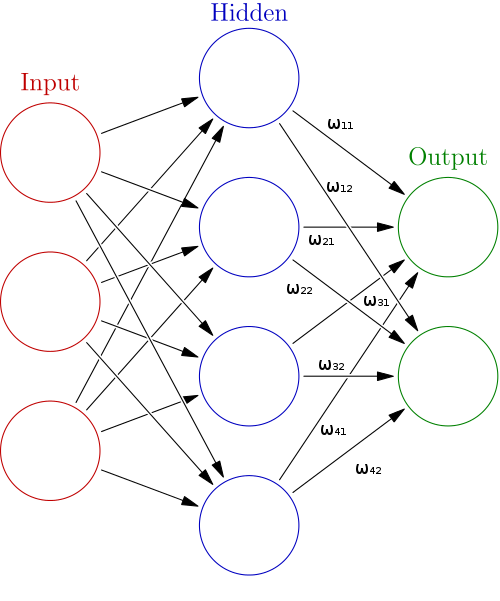
\includegraphics[scale=0.4]{structure2}
	\centering
	\end{figure}
  \begin{center}becomes\end{center}
\end{frame}

\begin{frame}{Matrices des poids}
	Transition entre couche la couche $i$ \`a $q$ neurones et couche $i+1$ \`a $p$ neurones:
	\[W_{i,i+1} = \begin{pmatrix}
		\omega_{11} & \omega_{21} & \cdots & \omega_{q1}\\
		\vdots & \vdots & \ddots & \vdots\\
		\omega_{1q} & \omega_{2q} & \cdots & \omega_{pq}\\
	\end{pmatrix} \in \mathscr{M}_{p,q}(\mathbb{R})\]

	Avec $\omega_{kl}$ le poids entre la neurone $k$ de la couche $i$ et $l$ de la couche $i+1$
\end{frame}

\begin{frame}{Forward Propagation}
	\begin{figure}
  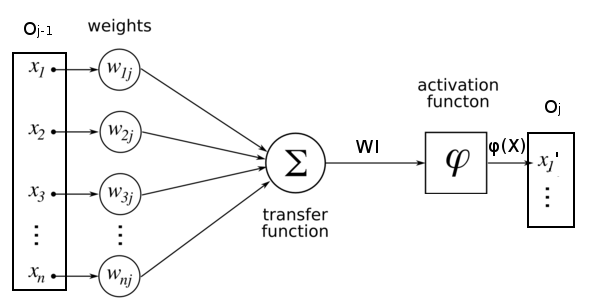
\includegraphics[scale=0.4]{forwardP2}
	\centering
	\end{figure}

	\[O_j=\varphi(W_{j-1,j}\times O_{j-1})\]
\end{frame}

\begin{frame}{Fonctions d'activation}
  \begin{figure}
    \begin{tikzpicture}
      \begin{axis}[
		no marks,
        mlineplot,
        width=0.9\textwidth,
        height=5.5cm,
		xlabel={x},
		ylabel={f(x)},
		title={Fonction sigmo\"ide et \'echelon},
		legend style={at={(0.40,0.85)}}
		]

		\addplot+ {1/(1 + e^(-x))};
		\addplot[domain=-5:0,brown] {0};
		\addplot[domain=0:5,brown] {1};
		\draw[dotted,brown] (axis cs:0,0) -- (axis cs:0,1);
		\addplot[soldot] coordinates{(0,0)};
		\addplot[holdot] coordinates{(0,1)};

      \legend{$x \mapsto \frac{1}{1 + e^{-x}}$, 
		$x \mapsto \begin{cases} 
			0 & x\leq 0 \\
			1 & x>0
   \end{cases}$ }

      \end{axis}
    \end{tikzpicture}
  \end{figure}
\end{frame}

\begin{frame}{Backpropagation}
	\[X = W^T E\]
\end{frame}

\begin{frame}{Training}
	\[\frac{\partial E}{\partial \omega_{jk}} = - (t_k - o_k) \times \varphi\left(\sum_j \omega_{jk} \times o_j\right)
	\left[1-\varphi\Big(\sum_j \omega_{jk} \times o_j\Big)\right]\times o_j\]	
\end{frame}

\begin{frame}{Blocks}
  Three different block environments are pre-defined and may be styled with an
  optional background color.

  \begin{columns}[T,onlytextwidth]
    \column{0.5\textwidth}
      \begin{block}{Default}
        Block content.
      \end{block}

      \begin{alertblock}{Alert}
        Block content.
      \end{alertblock}

      \begin{exampleblock}{Example}
        Block content.
      \end{exampleblock}

    \column{0.5\textwidth}

      \metroset{block=fill}

      \begin{block}{Default}
        Block content.
      \end{block}

      \begin{alertblock}{Alert}
        Block content.
      \end{alertblock}

      \begin{exampleblock}{Example}
        Block content.
      \end{exampleblock}

  \end{columns}
\end{frame}

\section{Analyse}

\begin{frame}{R\'esultats}
  \begin{table}
    \caption{R\'esultats du r\'eseau de neurones artificiels}
    \begin{tabular}{lr}
      \toprule
      Nombre exemples & $60000$\\
	  Nombre tests & $10000$\\
      %\midrule
      CA & 0.3\\
      Couches  & 3\\
      Nombre neurones & 100\\
      Performance & 0.94\\
      \bottomrule
    \end{tabular}
  \end{table}
\end{frame}

\begin{frame}{Coefficient d'apprentissage}
  \begin{figure}
    \begin{tikzpicture}
      \begin{axis}[
        mlineplot,
        width=0.9\textwidth,
        height=6cm,
		xlabel={coefficient d'apprentissage},
		ylabel={performance},
		xmin=0, xmax=1, ymin = 0.85, ymax=1,
		title = {Influence du CA (100 neurones)},
      ]

        %\addplot {sin(deg(x))};
		\addplot plot coordinates {(0.01,0.9164) (0.05, 0.9438) (0.1, 0.9490) (0.2, 0.9486) (0.3, 0.9428) (0.4, 0.9330) (0.5, 0.9202) (0.6, 0.9045) (0.7, 0.8912) (0.8,0.8771) (0.9, 0.8565)};
        %%\addplot+[samples=100] {sin(deg(2*x))};

      \end{axis}
    \end{tikzpicture}
  \end{figure}
\end{frame}

\begin{frame}{Nombre neurones}
  \begin{figure}
    \begin{tikzpicture}
      \begin{axis}[
        mlineplot,
        width=0.9\textwidth,
        height=6cm,
		xlabel={Nombre neurones},
		ylabel={performance},
		xmin=0, xmax=400, ymin = 0.85, ymax=1,
		title = {Influence du nombre de neurones (CA = 0.1)},
      ]

        %\addplot {sin(deg(x))};
		\addplot plot coordinates {(20,0.9075) (50,0.9367) (80,0.9461) (110,0.9501) (140, 0.9530) (170,0.9549) (200,0.9564) (230,0.9573) (260,0.9577) (290,0.9582) (320,0.9582) (350,0.9585) (380,0.9589)};
        %%\addplot+[samples=100] {sin(deg(2*x))};

      \end{axis}
    \end{tikzpicture}
  \end{figure}
\end{frame}

\begin{frame}{Nombre it\'erations}
  \begin{figure}
    \begin{tikzpicture}
      \begin{axis}[
        mlineplot,
        width=0.9\textwidth,
        height=6cm,
		xlabel={Nombre it\'erations},
		ylabel={performance},
		xmin=0, xmax=10, ymin = 0.85, ymax=1,
		title = {Influence du nombre d'it\'erations}
      ]

        %\addplot {sin(deg(x))};
		%\addplot plot coordinates {(20,0.9075) (50,0.9367) (80,0.9461) (110,0.9501)};
        %%\addplot+[samples=100] {sin(deg(2*x))};

      \end{axis}
    \end{tikzpicture}
  \end{figure}
\end{frame}

\begin{frame}{Bar charts}
  \begin{figure}
    \begin{tikzpicture}
      \begin{axis}[
        mbarplot,
        xlabel={Foo},
        ylabel={Bar},
        width=0.9\textwidth,
        height=6cm,
      ]

      \addplot plot coordinates {(1, 20) (2, 25) (3, 22.4) (4, 12.4)};
      \addplot plot coordinates {(1, 18) (2, 24) (3, 23.5) (4, 13.2)};
      \addplot plot coordinates {(1, 10) (2, 19) (3, 25) (4, 15.2)};

      \legend{lorem, ipsum, dolor}

      \end{axis}
    \end{tikzpicture}
  \end{figure}
\end{frame}
\begin{frame}{Quotes}
  \begin{quote}
    Veni, Vidi, Vici
  \end{quote}
\end{frame}

{%
\setbeamertemplate{frame footer}{My custom footer}
\begin{frame}[fragile]{Frame footer}
    \themename defines a custom beamer template to add a text to the footer. It can be set via
    \begin{verbatim}\setbeamertemplate{frame footer}{My custom footer}\end{verbatim}
\end{frame}
}

\begin{frame}{References}
  Some references to showcase [allowframebreaks] \cite{knuth92,ConcreteMath,Simpson,Er01,greenwade93}
\end{frame}

\section{Conclusion}

\begin{frame}{Summary}

  Get the source of this theme and the demo presentation from

  \begin{center}\url{github.com/matze/mtheme}\end{center}

  The theme \emph{itself} is licensed under a
  \href{http://creativecommons.org/licenses/by-sa/4.0/}{Creative Commons
  Attribution-ShareAlike 4.0 International License}.

  \begin{center}\ccbysa\end{center}

\end{frame}

{\setbeamercolor{palette primary}{fg=black, bg=yellow}
\begin{frame}[standout]
  Questions?
\end{frame}
}

\appendix

\begin{frame}[fragile]{Backup slides}
  Sometimes, it is useful to add slides at the end of your presentation to
  refer to during audience questions.

  The best way to do this is to include the \verb|appendixnumberbeamer|
  package in your preamble and call \verb|\appendix| before your backup slides.

  \themename will automatically turn off slide numbering and progress bars for
  slides in the appendix.
\end{frame}

\begin{frame}[allowframebreaks]{References}

  \bibliography{demo}
  \bibliographystyle{abbrv}

\end{frame}

\end{document}
